\section{Intégration dans NewMadeleine}

TODO: toute cette section n'est pas faite

% algo des structure de données, Analyse des données, PAP Programantion des Architectures Parallèles pour le HPC, PDP Projet de Programmation pour le coté faire de la bibliographie, Lecture d'article et documentation scientifique, Langages du Parallélisme pour MPI...

\subsection{Présenté NewMadeleine details}

La bibliothèque de communications \emph{NewMadeleine} a donc plusieurs interfaces disponible pour l'utilisateur.
Les interfaces les puls important sont \emph{sendrecv} pour envoyer et recevoir des données,
\emph{coll} pour les opérations collective,
\emph{MPI} qui implémente le standard \emph{MPI} en utilisant les interface \emph{sendrecv} et \emph{coll},
\emph{rpc} qui permet le support des \emph{RPC}.

Pour ce stage nous avons utiliser principalement l'interface \emph{sendrecv}.
Ces interfaces permet a l'utilisateur de manipuler des requêtes de communications,
pour cela elles soumettre des tâches au core de la bibliothèque \emph{nm_core}.
Ces tâches sont de différant types comme : soumission d'une requêtes, completion des paquets, l'execution de handler...
Les tâches du core fonctionne dans des section critique donc utiliser une verrou nommé \emph{core_lock}.
La bibliothèque s'occupe automatiquement de la génération des requêtes et des paquets,
du découpage des données en tronçons et d'appliquer les stratégies d'optimisation.
Le core de la bibliothèque s'occuper de la progression des tâches et des communications grâce à la fonction \emph{nm_schedule}.
Cette fonction peut être déclancher à partir d'une interface (e.g. la fonction \emph{MPI_Test}).
Pour effectué les communications il est possible d'utiliser différant réseaux ou autre qui utilise une même interface, les drivers. % historiquement appelé minidriver
Lors de ce stage nous nous somme consentré sur les partis qui s'occupe des progression et sur les drivers,
donc nous ne rentrerons pas dans les détail sur les différante interfaces, sur les strategies, sur \emph{Pioman}, etc.

Dans les parties que nous avons manipuler lors du stage les paquets sont représenté par des "paquet wrapper",
nous allons les abréger \emph{pw} par la suite.
Les \emph{pw} posséde toute les informations pour l'envoi ou la réception de tronçons de données et pour que la tâche de completion de la requête puisse remonter les données à l'utilisateur.

La progression ce fait donc grâce à la fonction \emph{nm_schedule} qui :
\begin{itemize}
  \item commance par executer les tâches grâce à un verrou,
  \item puis elle fait progresser les \emph{pw} de réception,
  \item puis elle fait progresser les \emph{pw} d'envois,
  \item elle déclanche le préfetche si besoin,
  \item puis elle execute de nouveau les tâches dans le cas ou des nouvelles on étais soumisse par la progression de \emph{pw},
  \item et elle fini par envoyer si besoin des évenements au interfaces superieur
\end{itemize}

Tous les drivers suive une interface qui permet :

\begin{itemize}
  \item d'instancier le driver grâce à une fonction \emph{init} qui donne une url qui est partagé avec les autre processus pour initier une connection. % puk_context_t context
  \item d'instancier une connection grâce à une fonction \emph{connect} qui prend en paramètre l'url d'un autre processus avec qui on souhaite communiquer. % _status
  \item poster une réception ou un envois pour les trois type de représentation de données (iovec, buffer, data),
  seul un des types peut être implémenté dans le driver final.
  Les fonction sont \emph{send_XX_post} et \emph{recv_XX_post} avec les "XX" qui sont remplacé par les trois types \emph{iov}, \emph{buf} et \emph{data}.
  Nous utiliserons les terms \emph{poster une reception} et \emph{poster un envois} par la suite.
  \item scruté une réception ou un envois avec \emph{send_poll}, \emph{recv_poll_one} et \emph{recv_buf_poll}.
  Nous utiliserons les terms \emph{scruter une reception} et \emph{scruter un envois} par la suite.
  \item scruté une reception de n'importe quel source \emph{recv_probe_any}.
  \item libérer une connection et le driver en entier avec toutes les connections respectivement avec \emph{disconnect} et \emph{close}.
  \item diverse actions comme \emph{send_buf_get} pour récupérer l'adresse d'un nouveau buffer, \emph{recv_buf_release} pour le libérer, \emph{get_rdv_data} et \emph{set_rdv_data} pour les rendez-vous, etc...
\end{itemize}

Les trois différant type représente des données contigue pour le type "data" pour une zone alloué par l'utilisateur,
des données contigue pour le type "buffer" qui est une zone alloué par le driver et
des données non continue pour le type "iovec" qui représente un vecteur de plusieurs zone mémoire qui ne font pas forcément la même taille.

Un driver peut avoir plusieurs connections par instance.

Les paquets sont distinguer en deux categorie,
les petit qui rentre entierement dans l'espace mémoire utiliser pour la communication et
les gros qui ne rentre pas entiermment donc qui sont coupé en tronçons pour être envoyer un par un.
% req.data split in req_chunk

Les drivers on une instance différante pour les petit est les gos paquets.

Le core liste instances des drivers grâce à un \emph{nm_drv}.
Une instance d'un \emph{drv} possède une instance d'un driver pour les petit paquets,
une instance d'un driver pour les gros paquets et
possède des structure qui sont les même peut importe l'implémentation du driver,
c'est ce qui permet l'utilisation de différant implémentations de driver.
Lors de l'instanciation des \emph{drv} les drivers sont instancier, paramétré et leur url sont envoyer.
Donc nous distinguerons \emph{drv} et driver par la suite.

Le core possède deux liste de \emph{pw} pour la réception et pour l'envoi qui sont \emph{pending_send_list} et \emph{pending_recv_list}.
Ces liste possède :
\begin{itemize}
  \item un \emph{pw} par connections de chaque instance de driver,
  \item plus un \emph{pw} pour la liste de réception pour chaque instance de driver qui support les petit paquets et qui implémente la fonction \emph{recv_probe_any}.
  En effet seul les petit paquets peuvent avoir cette fonction.
  Le \emph{pw} supplémentaire est donc posté dans le cas ou l'on n'a pas poster de reception mais qu'on en reçois une.
\end{itemize}

Le \emph{pw} connais l'instance du driver au quel il est rattaché.
Dans le \emph{nm_schedule} faire progresser les \emph{pw} de réception consiste à parcourir chaque \emph{pw} de la liste de réception pour
poster une reception si besoin, faire un \emph{recv_probe_any} pour le \emph{pw} dédier et
scruter une reception pour les autre.
Si la scrutation est positive une tâche du core, abréger \emph{core_task}, de completion sera soumisse.
Quand le \emph{nm_schedule} fait progresser les \emph{pw} d'envois le fonctionnement est similaire à la réception sans le \emph{recv_probe_any}.

Le polling ce fait donc par des appels régulier à \emph{nm_schedule} depuis \emph{Pioman}, des appels à \emph{MPI_Test} ou \emph{MPI_Wait}.

J'ai eu des difficulté de compréhension pour le cycle de vide des \emph{pw} qui est un peut complex car il passe à pleins d'endrois (les listes, les core task, il sont réutilisé quand la tâche est traité...)

\subsection{Modification}

\subsubsection{Ajoute des driver}

Lors de ce stage on ce consentre donc sur le driver qui fait les communication en mémoire partagé,
nous l'appeleron \emph{driver shm}.

Nous avons donc ajouter deux drivers basé sur le driver \emph{shm}.
Un avec les signaux, driver \emph{sig_shm},
qui utilise les signaux comme abstraction des uintr.
Ce driver \emph{sig_shm} à étais très utile quand nous n'avions pas accès à la machine qui supporte les \uintr{},
et pour le debug.
Un second avec les \uintr{}, driver \emph{uintr_shm}, qui utilise donc les uintr.

C'est deux drivers initialise leur handler à l'initialisation (\emph{init}) et libérer la mémoire à la terminaison (\emph{close}).
Ce handler, de signal ou d'interruptions, leur est propre et permet de verifier si un handler de driver est défini et de l'appelé.
Un \emph{handler de driver} est un nouveau type de handler qui est définir par une fonction, \emph{set_handler} que nous avons ajouter à l'interface des drivers.
Cette fonction est appelé lors de l'instanciation du \emph{drv} juste après avoir instencier le driver et si le driver support les \emph{handler de driver}.
Le \emph{handler de driver} qui est donné par le \emph{drv} et defini dans le \emph{drv} et permet de faire la procession,
nous le verrons dans la section \ref{progression}.

Ces deux drivers on deux variantes, une pour les petit paquets et une pour les gros paquets.
Pour les signaux on utilise \emph{SIGUSR1} pour les petit paquets et \emph{SIGUSR2} pour les gros paquets avec un handler de signal chacun.
Pour les \uintr{} on utilise le vecteur 6 pour les petit paquets et 8 pour les gros paquets,
On neu peut défini qu'un handler pour les deux donc nous avons ajouté un module qui permet d'appelé un handler local au driver à partir d'un handler global.
Chaque driver possède donc sont handler, de signal ou d'interruptions, local qui est en capacité d'appelé le \emph{handler de driver}.

Pour ajouter le driver avec les \uintr{} nous avons ajouter l'argument \emph{--enable-uintr} dans le \emph{configure} de \emph{NewMadeleine}
pour activer le support des \uintr{} seulement quand on à le compilateur et la machine qui les support.
Nous avons aussi ajouter dans le \emph{Makefile.in} les bon flag de compilation.

L'envoi des signaux ou interruptions ce fait au moment de scruter une reception ou un envoi.
L'object final est que l'émetteur envois une interruption au récepteur pour l'avertir qu'il peut faire une scrutation,
le réceptuer fait ça scrutation et envois une interruption à l'émetteur pour le prévenir qu'il peut reçevoir la suite.
Dans le cas des petit paquets l'émetteur ne renvois pas d'interruption car la communication est finir par-contre
dans le cas des gros paquets le c'est allez-retour ce font j'usqu'a la fin de la communication.
On ce retouve donc à faire des scrutation seulement quand cela est nécessaire.

Actuellement on on envois une interruption ou un signal seulement au moment de scruter l'envoi
car le support des gros paquets ne focntionne pas encore.

On fait l'envois de l'interruption au moment de scruter car la bibliothèque scrute forcément après avoir posté une communication.

\subsubsection{Faire la progression à partir des handler}
\label{progression}

Pour fair progresser les communication à partir des handler est non par des scrutations répété on
commance par ne plus ajouter les \emph{pw} qui sont lié à un driver qui posséde un \emph{handler}.
On ajoute deux nouvelles liste de \emph{pw} pour la réception et pour l'envoi dans le \emph{drv} qui seront utilisé par le \emph{handler de driver}.
Ce \emph{handler de driver} qui est défini dans le \emph{drv} et est nommé \emph{drv_handler}.
Il est déclancher par le handler local des drivers.

Lors du déclanchement il connais l'instance du \emph{drv} et il vas effectuer une progression.
Ce handler commance par faire progresser les tâches du core si possible.
Comme il faut prendre le verrou \emph{core_lock} on vas essayer de le prendre avec la fonction \emph{try_lock}.
Si le lock peut être pris alors les tâches progresse sinon on passe.
Pour rappelle on ne peut pas attendre dans un handler de signal ou d'interruption et c'est bien ce genre de handler qui déclanche
le \emph{handler de driver}.

Ensuite on vas essayer de faire progresser tous les éléments de la nouvelles liste de \emph{pw}.
Pour ce faire on appel les même fonctions que le \emph{nm_schedule} principale.
On as modifier ces fonction pour quelle utilise les bonne liste en fonction de si le \emph{pw} support les handler ou non.
Avant de passer à la progression de l'éléments suivants on fait progresser les tâches du core si possible.
Si ce n'ai pas possible on ajoute l'instance du \emph{drv} dans une nouvelle file de \emph{drv} en attente (\emph{pending_drv}) qui ce trouve dans le core.

Une fois qu'on à fait progresser tous les éléments une fois on peut déterminé si il faut le faire une nouvelle fois.
Pour ce faire il faut que les tâches du core est pus progresser pour que les \emph{pw} sois disponible et que il sois nécessaire de faire une seconde progression.
Il est important de savoir que nous somme limité en nombre de \emph{pw} car nous ne pouvons pas fait d'allocation dans un handler de signal ou d'interruption
car une allocation, avec \emph{malloc} par example, n'est pas "async safe" donc peut attendre et on ne peut pas.

Une seconde progression est nécessaire dans le cas ou plusieurs interruption on étais reçus en même temps.
Nous ne pouvons pas savoir combien d'interruption on été reçus car elle s'écrase donc
on utilise la fonction \emph{recv_probe_any} du driver per determiner si il faut refaire une progression.
L'utilisation de \emph{recv_probe_any} fonctionne seulement pour les driver pour les petit paquets,
pour les drivers des gros paquets on fait qu'une seul progression pour le moment.
Le support des gros paquets n'ai pas terminé et fait l'objet de bugs.

Nous avons donc vue que nous utilison une file de \emph{drv} en attente car une partie des progression ce fait dans une zone critique et
que nous ne pouvons pas attendre dans un handler donc nous ne pouvons pas garantir le fait de prendre un verrou.

Les \emph{drv} de cette liste sont traité au moment où un thread relache le verrou du core ou quand on reçois de nouveau une interruption.
Le fait de traité les progression des \emph{drv} peut amener à des conflic si le handler ce déclanche et
fait également une progression donc il faut protégé cette progression.
Pour ce faire nous avons utiliser l'operation atomique \emph{compare and swap} pour s'assuré d'être seul à faire la progression.
Si le handler échoue le \emph{compare and swap} alors il ajoute l'instance du \emph{drv} à la file de \emph{drv} en attente.

\subsubsection{File de \emph{drv} en attente}

La file de \emph{drv} en attente est une file dons les operation d'enfiler et de défilé (enqueue et dequeue) sont se fon sans verrou (\emph{lock-free}).
C'est file \emph{lock-free} sont donc beaucoup utilisé dans \emph{NewMadeleine}.
Le principe de fonctionnement et de déterminer si quelqu'un d'autre modifie la file en même temps et si c'est le cas on attends.
On vois donc une problématique apparétre, elle attend.
Lors de nos test on ce retouve donc dans des états bloquant (deadlock en anglais).
Cette états bloquant est du au fait que l'on interronp le thread qui est entrais de moddifer la file et
le handler veut modifier la file aussi et donc attend que le thread interrompu est fini, ce qui n'arrive jamais du coup.
Pour résoudre ce problème il nous faut donc une file sans attente (\emph{wait-free}).

\subsubsection{File \emph{lock-free} et \emph{wait-free}}

J'ai donc fait de la bibliographie pour touver une implémentation dans la literature.

L'origine des file \emph{wait-free} viens des file \emph{lock-free}.
La premier file \emph{lock-free} est celle de Michael \& Scott \cite{MICHAEL19981} qui est nommé \emph{MSQueue} dans la literature.
Une premier file \emph{wait-free} qui est basé sur le même fonctionnement que la \emph{MSQueue} est proposé par A. Kogan \& E. Petrank \cite{10.1145/1941553.1941585},
Cette file est nommé \emph{KPQueue}. Elle à des performances très limité et ne passe pas à l'échelle.
Plusieurs autre file on été proposé pour amélioré les performances comme la \emph{FCQueue} de D. Hendler \& I. Incze \& N. Shavit \& M. Tzafrir \cite{10.1145/1810479.1810540},
Elle est \emph{wait-free} grâce à des verrou est à des performances résonable mais elle est basé sur des liste chainai ce qui veut dire que les éléments sont alloué à l'insertion
et on ne peut pas utiliser d'allocateur dans un handler d'interruption donc elle ne nous convien pas.
Les file \emph{CCQueue} et \emph{H-Queue} sont basé sur la même idée que la file \emph{FCQueue} mais peut passé à l'échelle,
elles sont proposé par P. Fatourou \& N. D. Kallimanis \cite{10.1145/2370036.2145849} mais pose les même problème que la \emph{FCQueue}.
La file \emph{SimQueue} (aussi nommé \emph{FKQueue}) est une file \emph{lock-free} et \emph{wait-free} qui est basé sur des liste chainai
donc nous convien pas en plus elle est moins performante que la file \emph{FCQueue}.
Elle a aussi des problèmes de liberation mémoire comme décrit par P. Ramalhete \& A. Correia \cite{10.1145/3155284.3019022}.
Elle est proposé par P. Fatourou \& N. D. Kallimanis \cite{10.1145/1989493.1989549}.
Ces même auteur on proposé \emph{PSim} \cite{Fatourou2014} qui est basé sur \emph{SimQueue} mais en plus efficasse.
Il aurais les même problèmes de liberation de la mémoire toujours décrit par P. Ramalhete \& A. Correia.
L'accès à l'article est payant mais dans les article sortie plus réçament on peut voir qu'il à de relativement bonne performances.
Une autre file \emph{wati-free} qui a des très bonne performances est la \emph{WFQueue} (aussi nommé \emph{YMC queue}),
elle est proposé par C.Yang \& J. Mellor-Crummey \cite{10.1145/3016078.2851168}.
Elle est basé sur des liste chainai et aurais les même problèmes de liberation de la mémoire toujours décrit par P. Ramalhete \& A. Correia.
P. Ramalhete \& A. Correia présente une file nommé \emph{CRTurn} \cite{10.1145/3155284.3019022} qui est \emph{wait-free} et qui cherche à corriger les problèmes de réclamation mémoire.
Leur implémentation n'est pas très performante mais il discute d'une grande partie des file précédente et les regroupé dans un même dépo \emph{Github} avec un moyen pour mesuré leurs performances.
En 2019 R. Nikolaev propose une file seulement \emph{lock-free} nommé \emph{SCQ} \cite{10.4230/lipics.disc.2019.28}
qui est inspiré sur une \emph{CRQ} mais qui est plus plus efficace en termes de mémoire et évite les problèmes de \emph{livelocks}.
\emph{CRQ} est une file \emph{lock-free} qui est performante est utilise l'operation atomique \emph{compare and swap}
sur 2 mots contigus mémoire \emph{CAS2} qui n'est pas disponible sur tous les CPU.
\emph{CRQ} est porposé par A. Morrison \& Y. Afek \cite{10.1145/2517327.2442527}.
\emph{SCQ} n'utilise pas les \emph{CAS2} et arrive à des performance similaire au \emph{CRQ}.
\emph{SCQ} passe également très bien à l'échelle.
En 2022 la file \emph{wCQ} qui basé sur \emph{SCQ} et qui est en plus \emph{wait-free} est proposé par R. Nikolaev \& B. Ravindran \cite{10.1145/3490148.3538572}
Elle est performante, passe très bien à l'échelle, les auteurs ce sont basé sur le dépo \emph{Github} de P. Ramalhete \& A. Correia
pour y ajouter leur implémentaion dans ce nouveau dépo \cite{wCQ}.

Pendent mes recherche mon tuteur de stage, \emph{Alexandre Denis} à amélioré sont implémentaion de la \emph{lfqueue} pour "\emph{Lock-Free} Queue".
Les éléments qui peuvent allez dans ça file sont des pointeur.
Il utilise une technique très astucieuse qui consite à utiliser les 16 premier bits non utiliser des pointeurs
compté le nombre de modification qu'a eu une entré de la file, et si il y a eu un changement entre la lecture et
l'écriture atomique il sais que quelqu'un d'autre modifie la liste est il peut réagire en conséquance.
Il a plusieurs variantes et je ne suis pas sur de pourvoir bien les expliquer.
Dans tous les cas cette implémentation feura l'objet d'une publication future.
Son implémentation serai mailleur que la \emph{wCQ} avec peut de thread et peut de contention et
un peut moins bonne dans les autre cas mais tous ceci est en cours de test.

L'amélioration de la \emph{lfqueue} nous à permis de corriger les deadlock.

% parlé des écheque avec les instance de connection (_status) au lieu des p_drv pour la pending_drv

\subsection{Suite de testes}

\emph{NewMadeleine} possède une suite de tests très complete qui test toutes ses interfaces, la charge, etc.
Nous avons donc executer la suite de tests après nos modification. Environ 87 tests passe sur les 93.
Les tests qui ne passe pas sont généralement les collective qui engendre beaucoup de communications et certains test rpc,
ces tests appel du code utilisateur qui peut utiliser des fonction non "async safe" et donc posé un problème avec le handler d'interruption.
Le fait que ces tests ne passe pas est du un problèmes de modification concurrent des "pw".
Nous avons une solution temporaire où l'on masque les interruptions qui nous permet de passer tous les tests sauf certain rpc.
Ce bug reste donc à corriger.

\subsection{Reste à faire et les bugs}

Il reste donc a corriger le bug de modification concurrente des "pw",
finir le support pour les gros paquets avec l'envois d'interruption au moment ou l'on scrute la réception et
le support de \emph{Pioman} pour la progression multithread.

Une communication de gros paquets commance toujours par un petit paquets pour l'entête puis passe à des gros paquets.
Actuellement le passage de petit à gros ne fonctionne pas correctement avec les interruptions, c'est peut être du au masquage.
Ce qui est sur c'est que le bug apparès aussi avec les signaux et lorsque l'on force l'envois d'un signal la communicaion ce fait bien,
c'est à dire les allez / retour de singaux, etc.

\subsection{Performances}

Nous avons donc mesuré les performances de nos drivers, pour ce faire nous avons utiliser les benchmark de \emph{NewMadeleine}.
Sur les résultats qui vont suivre nous allons nous concentrer seulement sur les taille de paquets (ou message) inferieur à 16ko qui correspond à la taille des petit paquets.

\subsubsection{Résultats avec attente active}

Le premier benchmark est \emph{nm_bench_sendrecv} qui mesure notamment la latence et le débit d'un allez-retour (ping-pong) en attend active.
Sur la figure \ref{fig:sendrecvBenchLatency} on peut voir les courbes de latence.

Sur l'axe des abscisses on vois la taille des paquets et sur l'axe des ordonnées la latence en microsecondes.
On vois avec la courbe bleus les performances du driver \emph{shm} qui fait seulement de l'attente active.
On vois avec la courge vert les performances du driver \emph{uintr_shm}, on peut remarquer que la latence est la même que pour le driver \emph{shm} avec la latence des \uintr{} en plus.
C'est ce qui est attendu car dans ce cas l'attente active à forcément le mailleur performances car elle ne fait que regardé si un paquet est reçus.
Et pour finir, on vois avec la courge orange les performances du driver \emph{sig_shm} qui on également la latence des signaux em plus et même un peut plus.

\begin{figure}[H]
  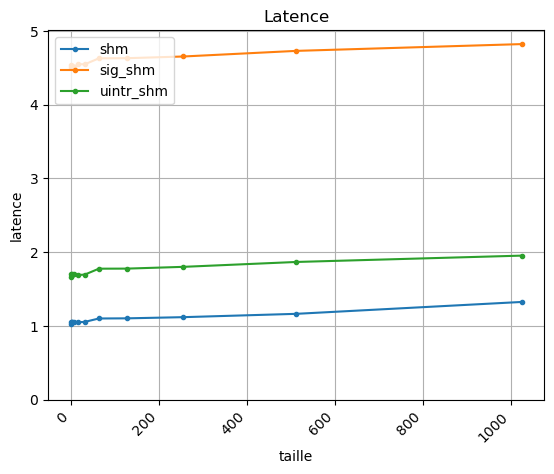
\includegraphics[width=\textwidth]{sendrecvBenchLatency}
  \caption{Latence avec le benchmark sendrecv}
  \label{fig:sendrecvBenchLatency}
\end{figure}

Sur la figure \ref{fig:sendrecvBenchThroughput} on vois les courbes de débit.
Sur l'axe des abscisses on vois la taille des paquets et sur l'axe des ordonnées le débit en Mo par seconde.
On peut voir grâce à ces courbes de débit que le surcoût est constant.

\begin{figure}[H]
  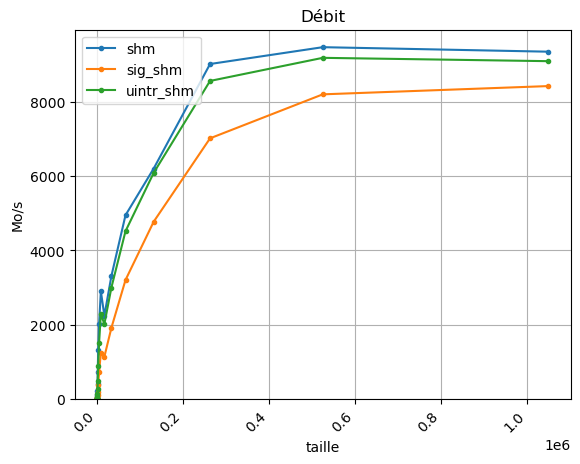
\includegraphics[width=\textwidth]{sendrecvBenchThroughput}
  \caption{Débit avec le benchmark sendrecv}
  \label{fig:sendrecvBenchThroughput}
\end{figure}

Ce cas d'attente active est peu représentatif des vrais application ou l'on cherche à recouvrir la latence des communications avec du calcule.
Donc on accèpte de perdre un peut en performances en attente active pour gagnier ailleur.

\subsubsection{Résultats recouvrement communication par du calcule}

Dans la plus part des application HPC on cherche à recouvrir la latence des communications avec du calcule, l'\emph{overlap} en anglais.
Le comportement que l'on cherche donc à avoir est que l'application fait du calcule et on l'interromp à un moment pour faire les communications.
On peut voir sur la figure \ref{fig:appPollingVsUintr} en annexe un example d'une application qui fait du polling en comparaison à une application qui utilise les \uintr{}.

Les figures qui suivent mesure l'\emph{overlap} au niveau de la réception car pour rapelle actuelleemnt seul le récepteur est interrompu.
Sur ces figures nous allons seulement nous concentrer sur la partie de gauche pour les taille de moins de 16ko.

Sur la figure \ref{fig:benchOverlapRecvShm} on peut voire un graphique sous forme de tuile qui représente la taille des message sur l'axe des abscisses
et le temps de calcule en microsecondes sur l'axe des ordonnées.
Les valeur dans les coins en haut à gauche et en bas à droit on tendence à être érroné à cause de la precision de la messure,
quand on envois très peut de données avec une temps de calcule très long il vas être complique de voire une différance de temps lier à l'envois.
Les couleur coresponde à un ratio du temps mesuré de l'execution moins le plus grand temps entre le temps de calcule et le temps de communicaion le tous normalisé à 1.
La couleur noire correspond donc à une valeur de 0 qui signifie que l'\emph{overlap} et parfait,
la couleur rouge correspond à 1 donc pas d'\emph{overlap} et
la couleur jaune correspond à 2 ou plus donc on est plus lent que si on n'avais pas essayer de faire d'\emph{overlap}.
Toutes les valeurs entre 0 et 1 qui passe du noire au violet pour arriver au rouge coresponde donc à un overlap plus ou moin présent.

Donc notre figure corespond au benchmark d'\emph{overlap} à la réception avec le driver \emph{shm}.
On peut voir qu'il y a pas vraiment d'overlap car c'est un driveur qui fait seulment de l'attente active.

\begin{figure}[H]
  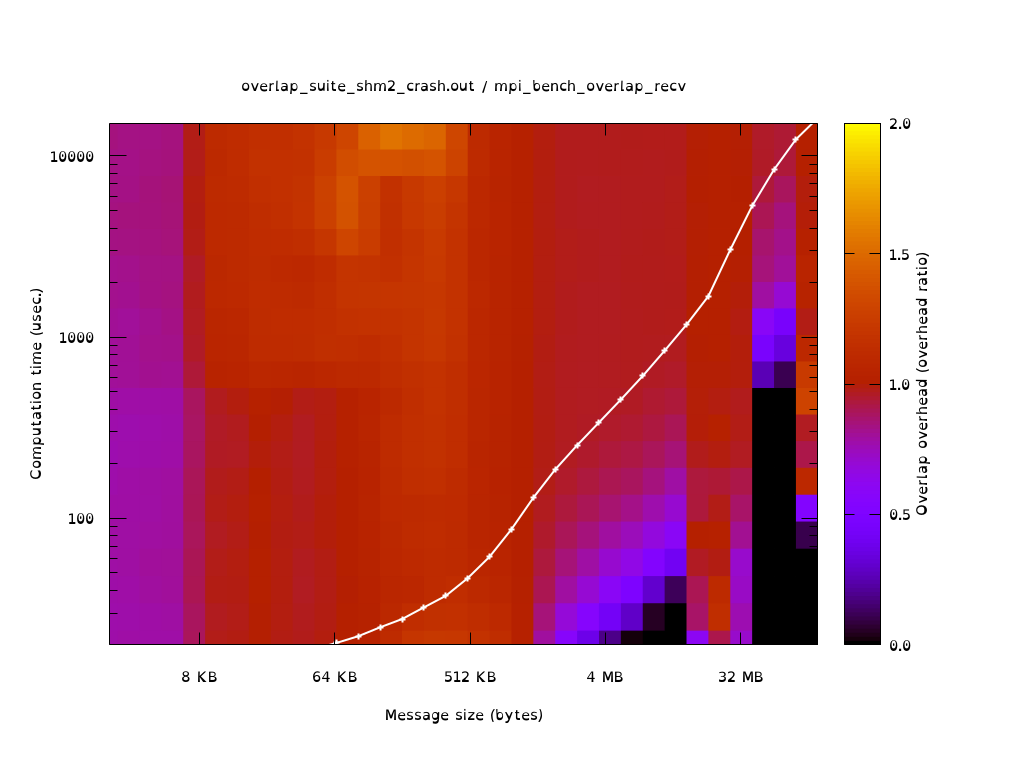
\includegraphics[width=\textwidth]{benchOverlapRecvShm}
  \caption{Benchmark d'overlap pour la réception avec le driver \emph{shm}}
  \label{fig:benchOverlapRecvShm}
\end{figure}

Sur la figure \ref{fig:benchOverlapRecvShmUintr} on peut voire un graphique qui corespond au benchmark d'\emph{overlap} à la réception avec le driver \emph{uintr_shm}.
On vois que pour les petit paquets, les messages plus petit que 16ko, l'\emph{overlap} et presque parfait et
même les plus grops paquets bénéficie d'une petite amélioration car le premier paquets d'entête passe par les petit paquets.
\begin{figure}[H]
  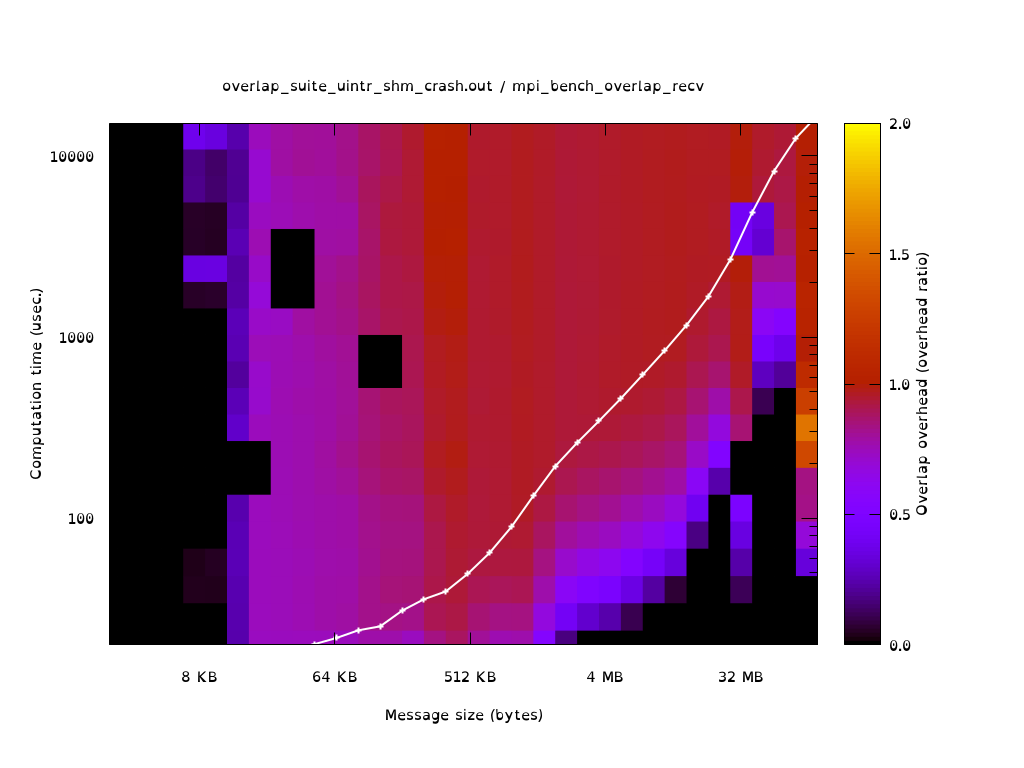
\includegraphics[width=\textwidth]{benchOverlapRecvShmUintr}
  \caption{Benchmark d'overlap pour la réception avec le driver \emph{uintr_shm}}
  \label{fig:benchOverlapRecvShmUintr}
\end{figure}

C'est resutats nous montre que l'utilisation d'\uintr{} permet bien de fait progresser le communications sans polling
avec des performances interrécente.
